\documentclass[../main.tex]{subfiles}
\graphicspath{{\subfix{../figures/}}}
%
\begin{document}
\section{桥梁模式(Bridge)}
桥梁模式虽然不是一种使用频率很高的模式,但是熟悉这个模式对于理解面向对象的设计原则,
包括开闭原则(OCP)以及组合聚合复用原则(CARP)都很有帮助.理解好这两个原则,有助于形成正确的设计思想和培养良好的设计风格.

\textbf{桥梁模式的目的}:将抽象化(Abstraction)与实现化(Implementation)脱耦,使得二者可以独立地变化.
%
\begin{itemize}
  \item \textbf{抽象化}:存在于多个实体中的共同的概念,就是抽象化.作为一个过程,抽象化就是忽略一些信息,从而把不同的实体当做同样的实体对待.
  \item \textbf{实现化}:对抽象化给出的具体实现,就是实现化.
  \item \textbf{脱耦}:
    \begin{enumerate}
      \item 所谓耦合,就是两个实体的某种强关联.而将它们的强关联去掉,就是耦合的解脱,或称脱耦.在这里,脱耦是指将抽象化和实现化之间的耦合解脱开,或者说是将它们之间的强关联改换成弱关联.
      \item 将两个角色之间的继承关系改为聚合关系,就是将它们之间的强关联改换成为弱关联.
    \end{enumerate}
\end{itemize}
%
因此,桥梁模式中的所谓脱耦,就是指在一个软件系统的抽象化和实现化之间使用组合/聚合关系而不是继承关系,从而使两者可以相对独立地变化.这就是桥梁模式的用意.

\textbf{以下的情况下应当使用桥梁模式}:
\begin{itemize}
  \item 如果一个系统需要的抽象化角色和具体化角色之间增加更多的灵活性,避免在两个层次之间建立静态关系.
  \item 设计要求实现化角色的任何改变不应当影响客户端,或者说实现化角色的改变对客户端是完全透明的.
  \item 一个构件有多于一个的抽象化角色和实现化角色,系统需要它们之间进行动态耦合.
  \item 虽然在系统中使用继承是没有问题的,但是由于抽象化角色和具体化角色需要独立变化,设计要求需要独立管理这两者.
\end{itemize}
%
\textbf{继承关系的缺点}:
继承存在不可避免的缺点,即灵活性不够.继承是一种强耦合,它在一开始便把抽象化角色和实现化角色的关系绑定(binding),使得两个层次之间互相限制,无法独立地演化.
那么,能否使用一种弱耦合来实现抽象化角色和实现者层次之间的动态绑定呢?
桥梁模式就提供了这样一种用聚合关系实现的弱耦合解决方案.
%
\subsection{桥梁模式的结构}
桥梁模式是对象形式的结构模式,又称为柄体(Handle and Body)模式或接口(Interface)模式. 下图所示就是一个实现了桥梁模式的示意性系统的结构图.
%
\begin{figure}[H]
  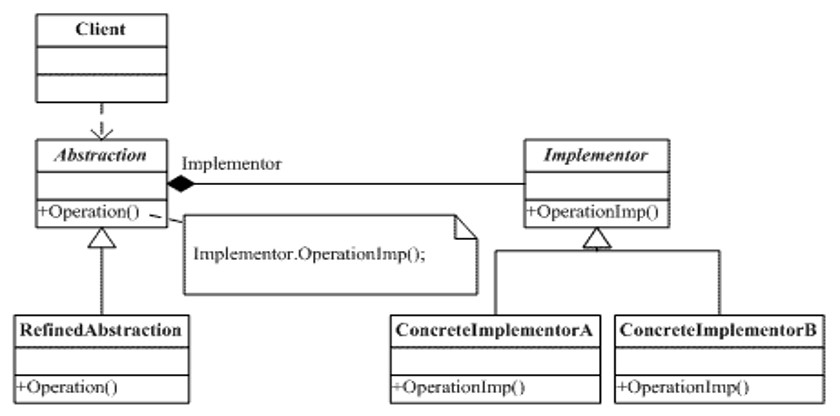
\includegraphics[width=0.60\textwidth]{26_1.jpg}
\end{figure}
%
这个系统含有两个等级结构:
%
\begin{itemize}
  \item 由抽象化角色和修正抽象化角色组成的抽象化等级结构.
  \item 由实现化角色和两个具体实现化角色所组成的实现化等级结构.
\end{itemize}
%
\textbf{桥梁模式涉及的角色}:
\begin{itemize}
  \item 抽象化(Abstraction)角色:抽象化给出的定义,并保存一个对实现化对象的引用.
  \item 修正抽象化(Refined Abstraction)角色:扩展抽象化角色,改变和修正父类对抽象化的定义.
  \item 实现化(Implementor)角色:这个角色给出实现化角色的接口,但不给出具体的实现.必须指出的是,这个接口不一定和抽象化角色的接口定义相同,实际上,这两个接口可以完全不同.实现化角色应当只给出底层操作,而抽象化角色应当只给出基于底层操作的更高一层的操作.
  \item 具体实现化(Concrete Implementor)角色:这个角色给出实现化角色接口的具体实现.
\end{itemize}
%
\lstinputlisting[language=java]{./code/26/1/Abstraction.java}
\lstinputlisting[language=java]{./code/26/1/RefinedAbstraction.java}
\lstinputlisting[language=java]{./code/26/1/Implementor.java}
\lstinputlisting[language=java]{./code/26/1/ConcreteImplementorA.java}
%
\textbf{接口的``宽''与``窄''}:
%
\begin{itemize}
  \item 一般而言,实现化角色中的每一个方法都应当有一个抽象化角色中的某一个方法与之相对应.
  \item 但是,反过来则不一定成立,即抽象化角色的接口比实现化的接口宽.
  \item 抽象化角色除了提供与实现化角色相关的方法外,还有可能提供其他的业务逻辑方法;而实现化角色则往往仅为实现抽象化角色的相关行为而存在.
\end{itemize}
%
\subsection{Java 中的Peer结构}
一个Java的软件系统总是带有所在的操作系统的视感(Look and Fell).如果一个软件系统是在UNIX上面开发的,那么开发人员看到的是Motif用户界面的视感;在Windows上面使用这个系统的用户看到的是Windows用户界面的视感;而一个在Macinto-sh上面使用的用户看到的则是Macintosh用户界面的视感.

在一个Java应用程序和真正的显示界面之间还有几个软件架构层次.假设现在考察的是一个Button构件,那么在屏幕上看到的是一个本地的按钮,与所在的操作系统的任何其他按钮并无区别.因为这个与系统有关的按钮实际上是Java的Button对象的Peer对象所产生的,这个对象的类型是java.awt.peer.Button ,而不是Java应用程序所使用的类型为java.awt.Button的对象.这个Peer对象会首先截获诸如鼠标单击这样的事件,然后将相关信息传递给java的按钮对象.
%
\begin{figure}[H]
  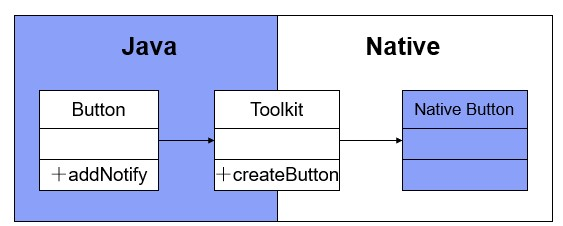
\includegraphics[width=0.45\textwidth]{26_2.jpg}
\end{figure}
%
这个将Java的GUI构件与本地环境的Peer构件联系起来的接口,就是所谓的Peer接口(ComponentPeer).
一个Peer接口其实就是一个定义了Peer构件必须实现的各个方法的接口.而AWT提供的所有Peer接口都放在java.awt.peer库中.比如这个库里有一个叫做ButtonPeer的接口,这个接口仅含有一个setLabel()的方法,

这意味着所对应的本地对象必须实现这个方法,才可以成为AWT的Peer对象.当然,正如Button本身还是Component的子类型,因而必须实现Component所规定的抽象方法一样,ButtonPeer本身还是ComponentPeer的子类型,所以必须实现ComponentPeer接口所规定的各个方法.两种颜色代表两个不同的等级结构.
%
\begin{figure}[H]
  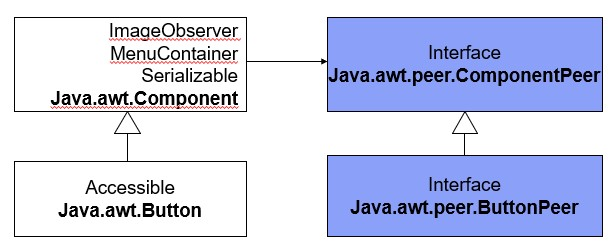
\includegraphics[width=0.45\textwidth]{26_3.jpg}
  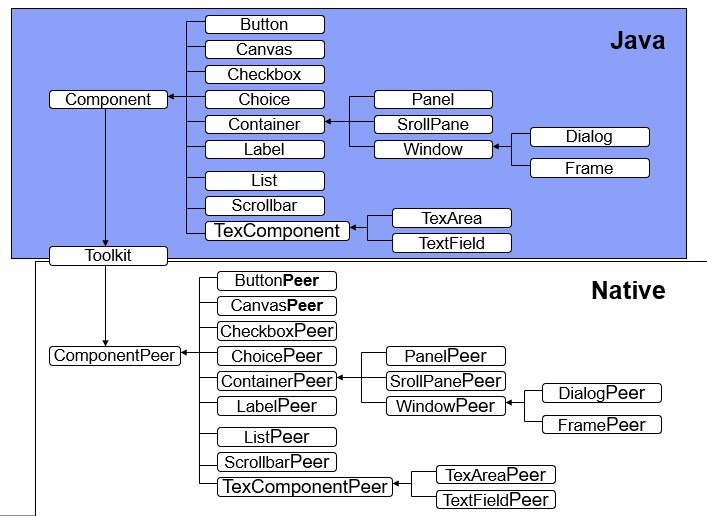
\includegraphics[width=0.55\textwidth]{26_4.jpg}
\end{figure}
%
\subsection{例子}
\noindent \textbf{问题}:空中客车(Airbus)、波音(Boeing)和麦道(donnell-Douglas)都是飞机制造商,它们都生产载客飞机(Passenger Plane)和载货飞机(Cargo Plane).现在需要设计一个系统,描述这些飞机制造商以及它们所造的飞机种类.

\noindent \textbf{设计方案一}:
首先,系统是关于飞机的,因此可以设计一个总的飞机接口,不妨叫做Airplane.其他所有的飞机都是这个总接口的子接口或者具体实现.
下图所示的就是这个设计方案的类图,可以看出,这是一个不大高明的设计,导致了一团理不清的关系.
%
\begin{figure}[H]
  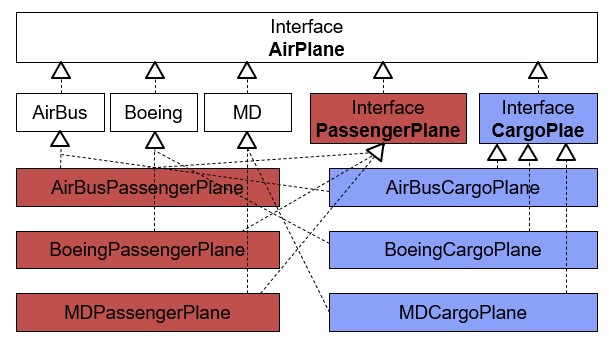
\includegraphics[width=0.55\textwidth]{26_5.jpg}
\end{figure}
%
可以看出,在这个设计方案里面,出现了两个子接口,分别表示客机和货机.所有的飞机又要继承自AirBus,Boeing和MD等超类.这样一来,每一个具体飞机都带有两个超类型:飞机制造商类型,客、货机类型.

\textbf{设计方案二}:
使用桥梁模式的关键在于准确地找出这个系统的抽象化角色和具体化角色.从系统面对的问题不难看出,代表飞机抽象化的是它的类型,也就是``客机''或者``货机'';而代表飞机的实现化的则是飞机制造商.
因此,可以给出一个更有灵活性的设计,这个使用了桥梁模式而做的新设计如下图所示.
%
\begin{figure}[H]
  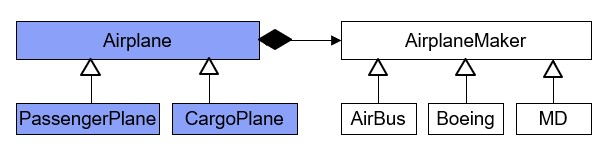
\includegraphics[width=0.55\textwidth]{26_6.jpg}
\end{figure}
%
首先Airplane扮演抽象化角色,它给出所有修正抽象化角色所需的接口, 它的源代码如下所示.
%
\lstinputlisting[language=java]{./code/26/2/Airplane.java}
%
载客飞机作为飞机种类,属于修正抽象化角色.它的示意性源代码如以下所示.
%
\lstinputlisting[language=java]{./code/26/2/PassengerPlane.java}
%
载货飞机作为飞机的另一个种类,也属于修正抽象化角色.它的示意性源代码如以下所示.
%
\lstinputlisting[language=java]{./code/26/2/CargoPlane.java}
%
飞机制造商AirplaneMaker扮演实现化角色,它给出所有的修正抽象化角色所需要实现的接口.它的源代码如以下所示.
%
\lstinputlisting[language=java]{./code/26/2/AirplaneMaker.java}
%
空中客车是飞机制造商之一,属于具体实现化角色.这里给出的是它的象征性Java源代码,如以下所示.
%
\lstinputlisting[language=java]{./code/26/2/Airbus.java}
%
波音是另一个飞机制造商,同样属于具体实现化角色.这里给出的是它的示意性Java源代码,如以下所示.
%
\lstinputlisting[language=java]{./code/26/2/Boeing.java}
%
同样地,飞机制造商麦道也属于具体实现角色,它的示意性Java源代码如下所示.
%
\lstinputlisting[language=java]{./code/26/2/MD.java}
%
\textbf{关于开闭原则(OCP)}:
现在,如果需要增加新的飞机种类,或者新的飞机制造商的话,只需要向系统引进一个新的修正抽象化角色,或者一个新的具体实现化角色就可以了.或者说,系统的功能可以在不修改已有代码的情况下得到扩展.
换言之,这个设计是符合开闭原则的.

\textbf{关于组合/聚合复用原则(CARP)}
由于这个新的系统设计适当地使用了继承关系来构建两个等级结构的内部结构,并且使用聚合关系来构建两个等级结构之间的关系,因此,这是一个通过使用``组合/聚合复用原则来达到开闭原则要求的范例.
%
\subsection{抽象与实现}
\textbf{对变化的封装}:
``找到系统的可变因素,将之封装起来'',通常就叫做``对变化的封装''.这实际上是达到``开-闭''原则的捷径,与组合/聚合复用原则是相辅相成的.
抽象化与实现化的最简单实现,也就是``开-闭''原则在类层次上的最简单实现,如下图所示.
%
\begin{figure}[H]
  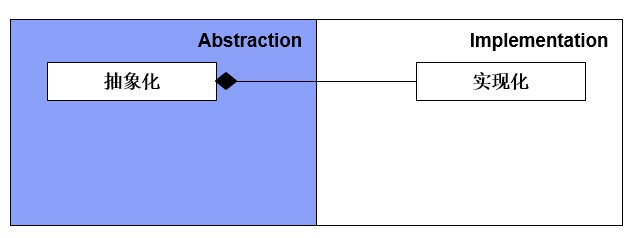
\includegraphics[width=0.50\textwidth]{26_7.jpg}
\end{figure}
%
一般来说,一个继承结构的第一层是抽象角色,封装了抽象的业务逻辑,这是系统中不变的部分.第二层是实现角色,封装了设计中会变化的因素.这个实现允许实现化角色有多态性变化,如下图所示.
%
\begin{figure}[H]
  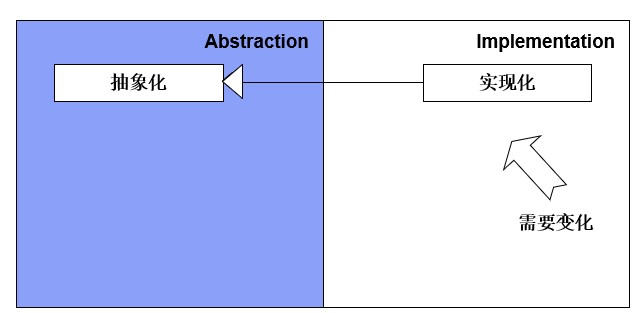
\includegraphics[width=0.50\textwidth]{26_8.jpg}
\end{figure}
%
换言之,客户端可以持有抽象化类型的对象,而不在意对象的真实类型是``实现化''、``实现化2''还是``实现化3'',如下图所示.
%
\begin{figure}[H]
  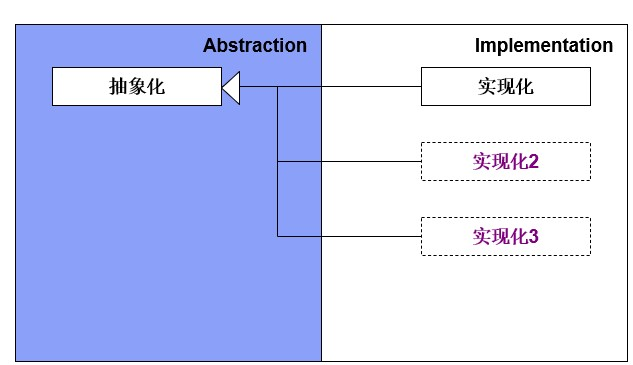
\includegraphics[width=0.50\textwidth]{26_9.jpg}
\end{figure}
%
显然,每一个继承关系都封装了一个变化因素,而一个继承关系不应当同时处理两个变化因素.这种简单实现不能够处理抽象化与实现化都面临变化的情况,如下图所示.
%
\begin{figure}[H]
  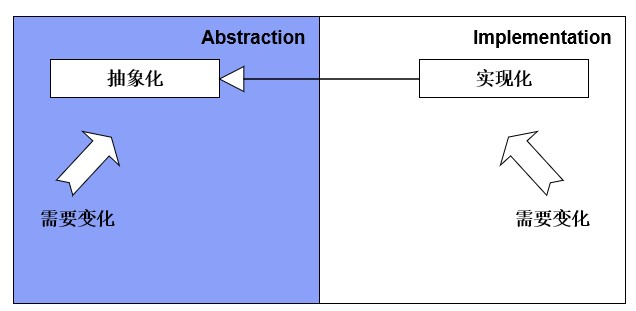
\includegraphics[width=0.50\textwidth]{26_10.jpg}
\end{figure}
%
上图的两个变化因素应当是彼此独立的,可以在不影响另一者的情况下独立演化.比如,下面的两个等级结构分别封装了自己的变化因素,由于每一个变化都是可以通过静态关系表达的,因此分别使用继承关系实现,如下图所示.
\begin{figure}[H]
  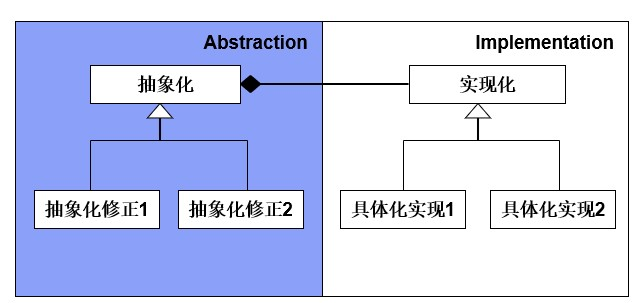
\includegraphics[width=0.50\textwidth]{26_11.jpg}
\end{figure}
%
\end{document}
